\documentclass[a4paper,10pt]{article}

% ============================================================================
% កញ្ចប់បណ្ណាល័យ (Packages)
% ============================================================================
\usepackage[a4paper, left=0.95cm, right=0.95cm, top=1.0cm, bottom=1.1cm, footskip=0.5cm]{geometry}
\usepackage{amsmath}
\usepackage{unicode-math}
\usepackage{fontspec}
\usepackage{array, longtable, multirow, colortbl}
\usepackage[table]{xcolor}
\usepackage{enumitem}
\usepackage{pifont}
\usepackage{fancyhdr}
\usepackage{tikz}
\usetikzlibrary{calc, arrows.meta, positioning, decorations.markings, babel}

% LaTeX 2025 + longtable v4.24 compatibility guard
\makeatletter
\let\@expl@@@mark@update@singlecol@structures@@\relax
\makeatother

% ============================================================================
% ការកំណត់ពុម្ពអក្សរឱ្យដូច Microsoft Word ១០០% (MS Word Fonts Configuration)
% ============================================================================
% Cross-platform font path resolver (Windows local + Linux/Cloud repo fonts/)
\providecommand{\NGSFindFonts}{%
  \IfFileExists{C:/Windows/Fonts/cambria.ttc}{%
    \def\NGSSysPath{C:/Windows/Fonts/}%
    \def\NGSUserPath{C:/Users/KIT/AppData/Local/Microsoft/Windows/Fonts/}%
  }{%
    \IfFileExists{./fonts/KhmerOSsiemreap.ttf}{\def\NGSSysPath{./fonts/}\def\NGSUserPath{./fonts/}}{%
    \IfFileExists{../fonts/KhmerOSsiemreap.ttf}{\def\NGSSysPath{../fonts/}\def\NGSUserPath{../fonts/}}{%
    \IfFileExists{../../fonts/KhmerOSsiemreap.ttf}{\def\NGSSysPath{../../fonts/}\def\NGSUserPath{../../fonts/}}{%
    \IfFileExists{../../../fonts/KhmerOSsiemreap.ttf}{\def\NGSSysPath{../../../fonts/}\def\NGSUserPath{../../../fonts/}}{%
    \IfFileExists{../../../../fonts/KhmerOSsiemreap.ttf}{\def\NGSSysPath{../../../../fonts/}\def\NGSUserPath{../../../../fonts/}}{%
    \IfFileExists{../../../../../fonts/KhmerOSsiemreap.ttf}{\def\NGSSysPath{../../../../../fonts/}\def\NGSUserPath{../../../../../fonts/}}{%
    \IfFileExists{../../../../../../fonts/KhmerOSsiemreap.ttf}{\def\NGSSysPath{../../../../../../fonts/}\def\NGSUserPath{../../../../../../fonts/}}{%
      \def\NGSSysPath{../../../../../../../fonts/}\def\NGSUserPath{../../../../../../../fonts/}%
    }}}}}}}%
  }%
}
\NGSFindFonts

\setmathfont[
  Path={\NGSSysPath},
  FontIndex=1,
  Scale=1.02
]{cambria.ttc}

\defaultfontfeatures{Ligatures=TeX}

\setmainfont[
  Path={\NGSUserPath},
  Extension=.ttf,
  Script=Khmer,
  BoldFont={KhmerOSsiemreap},
  BoldFeatures={FakeBold=1.8},
  ItalicFont={KhmerOSsiemreap},
  ItalicFeatures={FakeSlant=0.22},
  BoldItalicFont={KhmerOSsiemreap},
  BoldItalicFeatures={FakeBold=1.8, FakeSlant=0.22}
]{KhmerOSsiemreap}

\newfontfamily\muol[
  Path={\NGSUserPath},
  Extension=.ttf,
  Script=Khmer
]{KhmerOSmuollight}

\newfontfamily\NagaBold[
  Path={\NGSUserPath},
  Extension=.ttf
]{AKbalthom Naga Bold}

\newfontfamily\CalibriFont[
  Path={\NGSSysPath},
  Extension=.ttf
]{calibri}

\newfontfamily\CourierBullet[
  Path={\NGSSysPath},
  Extension=.ttf
]{cour}
\newcommand{\wcirc}{{\CourierBullet\fontsize{9.5pt}{11pt}\selectfont o}}

\XeTeXlinebreaklocale "km"
\XeTeXlinebreakskip = 0pt plus 1pt minus 0.1pt

% ============================================================================
% ការកំណត់ពណ៌ និងទម្រង់ទំព័រ (Colors & Page Style)
% ============================================================================
\definecolor{stepgray}{HTML}{D9D9D9}
\definecolor{headgray}{HTML}{F2F2F2}
\definecolor{boxgray}{HTML}{D9D9D9}
\definecolor{darkred}{HTML}{C00000}
\definecolor{red5e}{HTML}{FF0000}
\definecolor{triblue}{HTML}{DAE8FC}
\definecolor{triborders}{HTML}{6C8EBF}
\definecolor{arrowblue}{HTML}{4472C4}

\pagestyle{fancy}
\fancyhf{}
\renewcommand{\headrulewidth}{0pt}
\fancyfoot[R]{\CalibriFont\fontsize{11pt}{13pt}\selectfont\thepage}

\setlength{\parindent}{0pt}
\setlength{\parskip}{0pt}
\setlength{\tabcolsep}{3.8pt}

% ប្រភេទជួរឈរតារាងតម្រឹមឆ្វេង (Left-aligned table column type)
\newcolumntype{L}[1]{>{\raggedright\arraybackslash}p{#1}}

% ============================================================================
% ម៉ាក្រូជំនួយ (Helper Macros)
% ============================================================================
\newcommand{\fiveE}[1]{{\NagaBold\fontsize{9.5pt}{13pt}\selectfont\textcolor{red5e}{#1}}}
\newcommand{\timenote}[1]{\textcolor{darkred}{\textit{#1}}}
\newcommand{\redsub}[1]{\textcolor{darkred}{#1}}
\newcommand{\graybox}[1]{\colorbox{boxgray}{\strut\hspace{2pt}#1\hspace{2pt}}}
\newcommand{\ditem}{\tikz[baseline=-0.5ex]\fill (0,0.42ex) -- (0.42ex,0) -- (0,-0.42ex) -- (-0.42ex,0) -- cycle;\hspace{0.3em}}
\newcommand{\cnum}[1]{{\fontsize{10.5pt}{12pt}\selectfont\ding{\numexpr181+#1\relax}}\hspace{0.2em}}
\newcommand{\cfig}[1]{\par\vspace{4pt}{\centering #1\par}\vspace{4pt}}
\newcommand{\stepheader}[1]{\multicolumn{3}{|c|}{\cellcolor{stepgray}\muol #1} \\* \noalign{\hrule height 0.4pt}}
\newcommand{\fstrut}{\rule[-1.85ex]{0pt}{4.9ex}}
\newcommand{\topfstrut}{\rule{0pt}{3.8ex}}
\newcommand{\botfstrut}{\rule[-2.0ex]{0pt}{0pt}}

% ក្បាច់ក្រោមបាវចនា (Tacteing Flourish)
\newcommand{\khmflourish}{%
  
\begin{tikzpicture}[x=0.05bp, y=-0.05bp, baseline=0pt]
    \path[fill=black, nonzero rule]
      (847,-111) .. controls (867,-92) and (921,-137) .. (902,-147)
      .. controls (865,-168) and (826,-126) .. (803,-126)
      .. controls (750,-126) and (704,-146) .. (655,-143)
      .. controls (652,-129) and (616,-116) .. (612,-107)
      .. controls (616,-101) and (651,-89) .. (655,-74)
      .. controls (706,-73) and (747,-92) .. (804,-92)
      .. controls (825,-92) and (871,-48) .. (904,-72)
      .. controls (916,-81) and (866,-126) .. (847,-111)
      (1284,-108) -- (943,-122) -- (943,-97) -- (1284,-108)
      (426,-119) -- (78,-108) -- (426,-97) -- (426,-119)
      (522,-111) .. controls (502,-93) and (446,-136) .. (467,-147)
      .. controls (504,-168) and (543,-126) .. (566,-126)
      .. controls (594,-126) and (619,-118) .. (644,-136)
      .. controls (629,-158) and (612,-176) .. (592,-193)
      .. controls (629,-193) and (655,-163) .. (684,-143)
      .. controls (712,-164) and (739,-193) .. (776,-193)
      .. controls (757,-176) and (740,-157) .. (725,-136)
      .. controls (756,-112) and (783,-141) .. (821,-143)
      .. controls (801,-162) and (774,-192) .. (811,-192)
      .. controls (831,-175) and (849,-156) .. (864,-135)
      .. controls (876,-118) and (943,-114) .. (943,-111)
      .. controls (943,-104) and (876,-101) .. (864,-84)
      .. controls (849,-63) and (831,-44) .. (811,-27)
      .. controls (774,-27) and (801,-57) .. (821,-76)
      .. controls (783,-78) and (756,-107) .. (725,-83)
      .. controls (740,-61) and (757,-43) .. (776,-26)
      .. controls (739,-26) and (712,-55) .. (684,-76)
      .. controls (655,-56) and (629,-26) .. (592,-26)
      .. controls (612,-43) and (629,-61) .. (644,-83)
      .. controls (619,-101) and (594,-92) .. (566,-92)
      .. controls (544,-92) and (498,-48) .. (465,-72)
      .. controls (451,-82) and (502,-129) .. (522,-111)
      (684,-132) .. controls (661,-132) and (623,-115) .. (623,-109)
      .. controls (623,-101) and (663,-87) .. (684,-87)
      .. controls (706,-87) and (746,-101) .. (746,-109)
      .. controls (746,-115) and (708,-132) .. (684,-132)
      (684,-116) .. controls (675,-116) and (659,-112) .. (659,-109)
      .. controls (659,-105) and (676,-102) .. (684,-102)
      .. controls (693,-102) and (710,-105) .. (710,-109)
      .. controls (710,-112) and (694,-116) .. (684,-116);
  \end{tikzpicture}%
}

% ============================================================================
% ម៉ាក្រូគូសបន្ទាត់ចំនួន និងរូបភាពគណិតវិទ្យា (TikZ Math Diagram Macros)
% ============================================================================

% ១. គំនូសព្រួញផលគុណខ្វែង (Cross-multiplication diagram from Textbook p.3)
\newcommand{\drawCrossMult}{%
  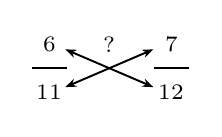
\begin{tikzpicture}[baseline=-0.5ex, scale=1.00, every node/.style={font=\footnotesize, text=black}]
    \node (n1) at (0, 0.30) {$6$};
    \node (d1) at (0,-0.30) {$11$};
    \draw[black, line width=0.6pt] (-0.22,0) -- (0.22,0);
    \node (n2) at (1.55, 0.30) {$7$};
    \node (d2) at (1.55,-0.30) {$12$};
    \draw[black, line width=0.6pt] (1.33,0) -- (1.77,0);
    \draw[{Stealth[scale=0.65]}-{Stealth[scale=0.65]}, line width=0.7pt, black] (0.20, 0.24) -- (1.32,-0.24);
    \draw[{Stealth[scale=0.65]}-{Stealth[scale=0.65]}, line width=0.7pt, black] (0.20,-0.24) -- (1.32, 0.24);
    \node[font=\footnotesize, text=black, fill=white, inner sep=1pt] at (0.76, 0.30) {$?$};
  \end{tikzpicture}%
}

% ២. បន្ទាត់ចំនួនក្នុងឧទាហរណ៍ ១ (Textbook p.3 Number Line: -1 to 1)
\newcommand{\drawTextbookNumberLine}[1][0.96]{%
  \begin{tikzpicture}[scale=#1, every node/.style={font=\footnotesize, text=black}]
    \draw[-{Stealth[scale=0.85]}, black, line width=0.8pt] (-3.65,0) -- (3.85,0);
    \foreach \x/\lbl in {
      -3.20/{-1},
      -2.40/{-0.75},
      -1.60/{-\frac{1}{2}},
      -0.80/{-0.25},
       0.00/{0},
       0.80/{\frac{1}{4}},
       1.60/{0.5},
       2.40/{\frac{3}{4}},
       3.20/{1}
    } {
      \draw[black, line width=0.65pt] (\x,-0.10) -- (\x,0.10);
      \node[above=3pt, font=\footnotesize, text=black] at (\x,0.08) {$\lbl$};
    }
  \end{tikzpicture}%
}

% ៣. បន្ទាត់ចំនួនសម្រាប់ឧទាហរណ៍ ២ (-9/7, -1, 1/8, 0.28, 1 2/5)
\newcommand{\drawExampleTwoLine}[1][0.98]{%
  \begin{tikzpicture}[scale=#1, every node/.style={font=\footnotesize, text=black}]
    \draw[{Stealth[scale=0.75]}-{Stealth[scale=0.85]}, black, line width=0.8pt] (-3.55,0) -- (3.70,0);
    % ក្រិតចំនួនគត់ -2, -1, 0, 1, 2
    \foreach \x/\n in {-3.20/-2, -1.60/-1, 0/0, 1.60/1, 3.20/2} {
      \draw[black, line width=0.65pt] (\x,-0.10) -- (\x,0.10);
      \node[below=3pt, font=\footnotesize, text=black] at (\x,-0.08) {$\n$};
    }
    % ចំណុចទាំង ៥៖ -9/7 (-1.285 -> -2.06), -1 (-1.60), 1/8 (0.125 -> 0.20), 0.28 (0.45), 1 2/5 (1.4 -> 2.24)
    \fill[black] (-2.06,0) circle (1.6pt);
    \node[above=4pt, xshift=-4pt, font=\footnotesize, text=black] at (-2.06,0.06) {$-\frac{9}{7}$};
    \fill[black] (-1.60,0) circle (1.6pt);
    \node[above=4pt, xshift=4pt, font=\footnotesize, text=black] at (-1.60,0.06) {$-1$};
    \fill[black] (0.20,0) circle (1.6pt);
    \node[above=4pt, xshift=-4pt, font=\footnotesize, text=black] at (0.20,0.06) {$\frac{1}{8}$};
    \fill[black] (0.45,0) circle (1.6pt);
    \draw[black, line width=0.5pt] (0.45,0.04) -- (0.78,0.28);
    \node[above, font=\footnotesize, text=black] at (0.88,0.26) {$0.28$};
    \fill[black] (2.24,0) circle (1.6pt);
    \node[above=4pt, font=\footnotesize, text=black] at (2.24,0.06) {$1\frac{2}{5}$};
  \end{tikzpicture}%
}

% ៤. រូបបន្ទាត់ចំនួនបង្ហាញចំនួនសនិទាននៅចន្លោះ 3/4 និង 6/7 (ឧទាហរណ៍ ៣)
\newcommand{\drawMidpointLine}[1][1.00]{%
  \begin{tikzpicture}[scale=#1, every node/.style={font=\footnotesize, text=black}]
    \draw[-{Stealth[scale=0.85]}, black, line width=0.8pt] (-3.0,0) -- (3.1,0);
    \draw[black, line width=0.65pt] (-2.0,-0.11) -- (-2.0,0.11);
    \draw[black, line width=0.65pt] ( 0.0,-0.11) -- ( 0.0,0.11);
    \draw[black, line width=0.65pt] ( 2.0,-0.11) -- ( 2.0,0.11);
    \fill[black] (-2.0,0) circle (1.6pt) node[above=3pt, font=\footnotesize, text=black] {$\dfrac{3}{4} = \dfrac{42}{56}$};
    \fill[black] ( 2.0,0) circle (1.6pt) node[above=3pt, font=\footnotesize, text=black] {$\dfrac{6}{7} = \dfrac{48}{56}$};
    \fill[black] ( 0.0,0) circle (1.8pt) node[above=3pt, font=\footnotesize, text=black] {$\dfrac{45}{56}$};
  \end{tikzpicture}%
}

% ============================================================================
% ចាប់ផ្ដើមឯកសារ (Document Body)
% ============================================================================
\begin{document}
\fontsize{10pt}{15.2pt}\selectfont

% -------------------- ក្បាលកិច្ចតែងការ (Header) --------------------
\begin{center}
  {\muol\fontsize{11pt}{16pt}\selectfont ព្រះរាជាណាចក្រកម្ពុជា}\\[2pt]
  {\muol\fontsize{10pt}{15pt}\selectfont ជាតិ សាសនា ព្រះមហាក្សត្រ}\\[1pt]
  \khmflourish
\end{center}

\vspace{-12pt}
{\muol\fontsize{10pt}{15pt}\selectfont អនុវិទ្យាល័យព្រះក្រសាំង}

\vspace{4pt}
\begin{center}
  {\muol\fontsize{10pt}{15pt}\selectfont កិច្ចតែងការបង្រៀន}
\end{center}
\vspace{2pt}

% -------------------- ព័ត៌មានទូទៅ (Metadata) --------------------
{\renewcommand{\arraystretch}{1.10}
\hspace*{4.6cm}%
\begin{tabular}{@{}l l l@{}}
  - \hspace{0.35cm} មុខវិជ្ជា & : & គណិតវិទ្យា ថ្នាក់ទី៨ (ពីជគណិត) \\
  - \hspace{0.35cm} ចំណងជើងមេរៀន & : & មេរៀនទី១ ចំនួនសនិទាន \\
  - \hspace{0.35cm} ចំណងជើងរង & : & ២. ការប្រៀបធៀប និងរៀបលំដាប់នៃចំនួនសនិទាន \\
  & & ២.២. ការរៀបលំដាប់ចំនួនសនិទាន \\
  - \hspace{0.35cm} រយៈពេល & : & ១ ម៉ោងសិក្សា (៤៥នាទី) \\
  - \hspace{0.35cm} បង្រៀនដោយ & : & ហុក ប៊ុនថែន \\
  - \hspace{0.35cm} កាលបរិច្ឆេទ & : & ០៤ វិច្ឆិកា ២០២៦ \\
\end{tabular}

\vspace{3pt}

% -------------------- I. វត្ថុបំណង --------------------
\textbf{I.} {\muol វត្ថុបំណង}\\[2pt]
\hspace*{0.55cm}%
\begin{tabular}{@{}l l l@{}}
  \wcirc \hspace{0.25cm} វិជ្ជាសម្បទា & : & សិស្សប្រាប់បានពីវិធីរៀបលំដាប់ចំនួនសនិទាន (ពីតូចទៅធំ ឬពីធំទៅតូច) និងការរកចំនួនសនិទាន \\
  & & នៅចន្លោះចំនួនសនិទានពីរបានត្រឹមត្រូវ តាមរយៈការសង្កេតបន្ទាត់ចំនួនលើក្ដារខៀន និងសំណួរបំផុស។ \\
  \wcirc \hspace{0.25cm} បំណិនសម្បទា & : & សិស្សរៀបលំដាប់ចំនួនសនិទាន (តាមបន្ទាត់ចំនួន ទសភាគ ឬតម្រូវភាគបែងរួម) និងគណនារកចំនួន \\
  & & សនិទាននៅចន្លោះចំនួនសនិទានពីរបានច្បាស់លាស់ តាមរយៈការធ្វើសន្លឹកកិច្ចការជាដៃគូ និងលំហាត់ប្រតិបត្តិ។ \\
  \wcirc \hspace{0.25cm} ចរិយាសម្បទា & : & សិស្សមានស្មារតីសហការ យកចិត្តទុកដាក់ និងមានទំនុកចិត្តក្នុងការបង្ហាញចម្លើយលើក្ដារខៀន \\
  & & តាមរយៈការពិភាក្សា និងអនុវត្តផ្ទាល់ជាមួយដៃគូក្នុងថ្នាក់។ \\
\end{tabular}

\vspace{1pt}

% -------------------- II. សម្ភារៈឧបទេស --------------------
\textbf{II.} {\muol សម្ភារៈឧបទេស}\\[1pt]
\hspace*{0.55cm}$\bullet$ \hspace{0.35cm} សៀវភៅសិក្សាគោលថ្នាក់ទី៨ (ទំព័រ ៣--៤) សន្លឹកកិច្ចការសិស្ស បណ្ណចំនួនសនិទាន បន្ទាត់វែង និងហ្វឺត/ដីសពណ៌

\vspace{1pt}

% -------------------- III. វិធីសាស្រ្តបង្រៀន --------------------
\textbf{III.} {\muol វិធីសាស្រ្តបង្រៀន}\\[1pt]
\hspace*{0.55cm}%
\begin{tabular}{@{}l l l@{}}
  $\bullet$ \hspace{0.35cm} គោលវិធី & : \hspace{0.7cm} & សិស្សមជ្ឈមណ្ឌល \\
  $\bullet$ \hspace{0.35cm} យុទ្ធវិធីបង្រៀន & : & ស្ថាបនានិយម គម្រូ 5Es (ការងារដៃគូ និងសន្លឹកកិច្ចការ) \\
\end{tabular}
}

\vspace{1pt}

% -------------------- IV. ដំណើរការបង្រៀន --------------------
\textbf{IV.} {\muol ដំណើរការបង្រៀន}

\vspace{1pt}

% ============================================================================
% តារាងដំណើរការបង្រៀន (Modular Multi-Row 3-Column Lesson Plan Table)
% បច្ចេកទេស៖ បំបែកតារាងជាជួរដេកតូចៗតាមផ្នែកនីមួយៗ (ដោយមិនដាក់ \hline នៅចន្លោះជួរតូចៗ)
% និងប្រើ \endhead / \endfoot ដើម្បីឱ្យ LaTeX បំពេញក្រដាសនីមួយៗឱ្យពេញ ១០០% ទើបឆ្លងទំព័រថ្មី។
% ============================================================================
\renewcommand{\arraystretch}{1.15}
\setlength{\LTpost}{2pt}
\begin{longtable}{|L{5.50cm}|L{7.90cm}|L{4.80cm}|}
\hline
\rowcolor{headgray}
\multicolumn{1}{|c|}{\muol សកម្មភាពគ្រូ} &
\multicolumn{1}{c|}{\muol ខ្លឹមសារមេរៀន} &
\multicolumn{1}{c|}{\muol សកម្មភាពសិស្ស} \\
\hline
\endfirsthead

\hline
\endhead

\hline
\endfoot

\hline
\endlastfoot

% ==================== ជំហានទី១ ====================
\stepheader{ជំហានទី១ (រដ្ឋបាលថ្នាក់)}
$\bullet$ ពិនិត្យអវត្តមានសិស្ស \par
$\bullet$ ពិនិត្យអនាម័យ និងសម្លៀកបំពាក់ \par
$\bullet$ ពង្រឹងវិន័យ និងសណ្ដាប់ធ្នាប់ក្នុងថ្នាក់
&
$\bullet$ រដ្ឋបាលថ្នាក់ \par
$\bullet$ អនាម័យថ្នាក់រៀន \par
$\bullet$ សណ្ដាប់ធ្នាប់ថ្នាក់រៀន
&
$\circ$ ប្រធានថ្នាក់រាយការណ៍ \par
$\circ$ រក្សាភាពស្ងៀមស្ងាត់ \\
\hline

% ==================== ជំហានទី២ ====================
\stepheader{ជំហានទី២ (កិច្ចការផ្ទះ +ទំនាក់ទំនងមេរៀនថ្មី)}
% --- ផ្នែក 2.1: កំណែកិច្ចការផ្ទះ (លំហាត់គំរូ ១ ទំព័រទី៣) ---
\timenote{ចំណាយពេលឱ្យតិចបំផុតកុំឱ្យលើស 3min} \par
$\bullet$ ពិនិត្យសៀវភៅកិច្ចការផ្ទះរបស់សិស្ស \par
$\bullet$ ហៅសិស្ស ២ នាក់ឡើងបំពេញចម្លើយកិច្ចការផ្ទះលើក្ដារខៀន
&
\centerline{\redsub{កំណែកិច្ចការផ្ទះ (លំហាត់គំរូ ១ ទំព័រទី៣)}} \par
១. បំពេញចន្លោះដោយសញ្ញា $( > , < , = )$ ចំពោះចំនួនខាងក្រោម៖
&
$\circ$ យកសៀវភៅកិច្ចការផ្ទះដាក់លើតុ \par
$\circ$ តំណាងសិស្ស ២ នាក់ឡើងបំពេញចម្លើយលើក្ដារខៀន \\[3pt]

&
\cfig{%
\begin{tabular}{@{}p{3.45cm}p{3.85cm}@{}}
  ក. $-6 \ \dots \ -3$ & ខ. $\fstrut\dfrac{-2}{7} \ \dots \ \dfrac{-5}{7}$ \\[4pt]
  គ. $\fstrut\dfrac{4}{3} \ \dots \ 1\dfrac{5}{7}$ & ឃ. $\fstrut 0.45 \ \dots \ \dfrac{54}{100}$
\end{tabular}}
& \\[3pt]

% --- ផ្នែក 2.2: ចម្លើយកំណែកិច្ចការផ្ទះ (ក និង ខ) ---
$\bullet$ សរសើរលើកទឹកចិត្តសិស្សដែលបានខិតខំធ្វើកិច្ចការផ្ទះបានត្រឹមត្រូវ
&
{\centering ដំណោះស្រាយ \par}
\begin{tabular}{@{}p{3.45cm}p{3.85cm}@{}}
  ក. $-6 < -3$ & ខ. $\fstrut\dfrac{-2}{7} > \dfrac{-5}{7}$
\end{tabular}
&
$\circ$ សង្កេត និងផ្ទៀងផ្ទាត់ចម្លើយលើក្ដារខៀន \\[3pt]

% --- ផ្នែក 2.3: ចម្លើយកំណែកិច្ចការផ្ទះ (គ និង ឃ) ---
$\bullet$ បញ្ជាក់បន្ថែមលើក្ដារខៀនអំពីការបំប្លែងចំនួនចម្រុះ $1\dfrac{5}{7}$ និងទសភាគ $0.45$ ទៅជាប្រភាគមុននឹងប្រៀបធៀប
&
\fstrut គ. $\dfrac{4}{3} = \dfrac{28}{21}$ និង $1\dfrac{5}{7} = \dfrac{7+5}{7} = \dfrac{12}{7} = \dfrac{36}{21}$ \par
\fstrut គេបាន $\dfrac{28}{21}$ និង $\dfrac{36}{21}$ ដោយ $36 > 28$ នាំឱ្យ \graybox{$\dfrac{4}{3} < 1\dfrac{5}{7}$} ។ \par
\fstrut ឃ. $0.45 = \dfrac{45}{100}$ និង $\dfrac{54}{100}$ \par
\fstrut ដោយ $45 < 54$ នាំឱ្យ \graybox{$0.45 < \dfrac{54}{100}$} ។
&
$\circ$ កែតម្រូវចំណុចខ្វះខាតចូលក្នុងសៀវភៅ \\[3pt]

% --- ផ្នែក 2.4: រំលឹកមេរៀនទាក់ទងមេរៀនថ្មី (ផលគុណខ្វែង ឧទាហរណ៍ ២ ទំព័រទី៣) ---
\timenote{ចំណាយពេលឱ្យតិចបំផុតកុំឱ្យលើស 1.5min} \par
$\bullet$ សរសេរប្រភាគ $\dfrac{6}{11}$ និង $\dfrac{7}{12}$ លើក្ដារខៀន \par
– \textbf{សំណួរ៖} តើប្រៀបធៀបដោយប្រើផលគុណខ្វែងដូចម្ដេច?
&
\centerline{\redsub{រំលឹកមេរៀនទាក់ទងមេរៀនថ្មី}} \par
$\bullet$ ការប្រៀបធៀបចំនួនសនិទានដោយផលគុណខ្វែង៖ \par
\ditem \textbf{ឧទាហរណ៍ ២ :} ចំនួនសនិទាន $\dfrac{6}{11}$ និង $\dfrac{7}{12}$
&
$\circ$ គណនាផលគុណខ្វែងផ្ទាល់មាត់៖ $6 \times 12 = 72$ និង $7 \times 11 = 77$ \\[3pt]

&
\cfig{\drawCrossMult}
& \\[3pt]

$\bullet$ ដឹកនាំសិស្សសរសេរការសន្និដ្ឋាន
&
$\bullet$ $6 \times 12 < 7 \times 11$ \par
$\bullet$ $72 < 77$ \hspace{0.2cm} ដូច្នេះ គេសន្និដ្ឋានថា \graybox{$\dfrac{6}{11} < \dfrac{7}{12}$} ។
&
$\circ$ ឆ្លើយថា $\dfrac{6}{11} < \dfrac{7}{12}$ \\[3pt]

% --- ផ្នែក 2.5: ប្រអប់ជាទូទៅនៃផលគុណខ្វែង ---
$\bullet$ ឱ្យសិស្សទាញរូបមន្តទូទៅនៃការប្រៀបធៀបប្រភាគពីរដែលមានភាគបែងវិជ្ជមាន
&
\cfig{%
{\setlength{\tabcolsep}{5pt}%
\renewcommand{\arraystretch}{1.20}
\begin{tabular}{|L{7.20cm}|}
  \hline
  \cellcolor{headgray}\fstrut\textbf{ជាទូទៅ :} ចំពោះចំនួនសនិទាន $\dfrac{a}{b}$ និង $\dfrac{c}{d}$ ដែល $b > 0$ និង $d > 0$ \\[2pt]
  \cellcolor{headgray}\fstrut\hspace*{0.25cm}- បើ $\dfrac{a}{b} < \dfrac{c}{d}$ នោះ $ad < bc$ \\[2pt]
  \cellcolor{headgray}\fstrut\hspace*{0.25cm}- ច្រាសមកវិញ បើ $ad < bc$ នោះ $\dfrac{a}{b} < \dfrac{c}{d}$ ។ \\[2pt]
  \hline
\end{tabular}}}
&
$\circ$ ឆ្លើយរូបមន្តទូទៅ៖ ចំពោះ $b>0, d>0$ បើ $ad < bc$ នោះ $\dfrac{a}{b} < \dfrac{c}{d}$ \\[3pt]

% --- ផ្នែក 2.6: រំលឹកពីបន្ទាត់ចំនួន ---
\timenote{ចំណាយពេលឱ្យតិចបំផុតកុំឱ្យលើស 1.5min} \par
$\bullet$ គូសបន្ទាត់ចំនួនលើក្ដារខៀន \par
– \textbf{សំណួរ៖} នៅលើបន្ទាត់ចំនួន តើចំនួនអវិជ្ជមាន និងចំនួនវិជ្ជមានស្ថិតនៅខាងណាគល់ $0$?
&
$\bullet$ ទីតាំងចំនួននៅលើបន្ទាត់ចំនួន (គូសលើក្ដារខៀន)៖
&
$\circ$ សង្កេតបន្ទាត់ចំនួនលើក្ដារខៀន \\[3pt]

&
\cfig{%
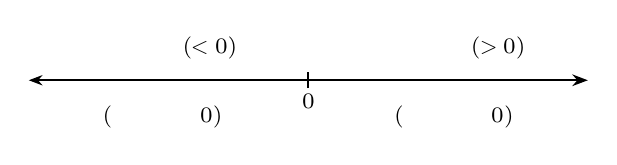
\begin{tikzpicture}[scale=1.00, every node/.style={font=\footnotesize, text=black}]
  \draw[{Stealth[scale=0.75]}-{Stealth[scale=0.85]}, black, line width=0.8pt] (-3.55,0) -- (3.55,0);
  \draw[black, line width=0.65pt] (0,-0.10) -- (0,0.10) node[below=4pt, font=\footnotesize, text=black] {$0$};
  \node[above=3pt, font=\footnotesize, text=black] at (-1.85,0.04) {ចំនួនអវិជ្ជមាន ($<0$)};
  \node[above=3pt, font=\footnotesize, text=black] at ( 1.85,0.04) {ចំនួនវិជ្ជមាន ($>0$)};
  \node[below=4pt, font=\footnotesize, text=black] at (-1.85,-0.06) {(នៅខាងឆ្វេងគល់ $0$)};
  \node[below=4pt, font=\footnotesize, text=black] at ( 1.85,-0.06) {(នៅខាងស្ដាំគល់ $0$)};
\end{tikzpicture}}
&
$\circ$ ឆ្លើយ៖ ចំនួនអវិជ្ជមាននៅខាងឆ្វេងគល់ $0$ និងចំនួនវិជ្ជមាននៅខាងស្ដាំគល់ $0$ \\[3pt]

% --- ផ្នែក 2.7: E1 - Engage ---
\fiveE{E1 - Engage (3min)} \par
$\bullet$ បិទបណ្ណចំនួនសនិទានទាំង ៥ លើក្ដារខៀន៖ \par
$\dfrac{1}{8}, -1, \dfrac{-9}{7}, 0.28, 1\dfrac{2}{5}$
&
$\bullet$ បណ្ណចំនួនសនិទានទាំង ៥ បិទលើក្ដារខៀន៖
&
$\circ$ សង្កេតបណ្ណចំនួនសនិទានលើក្ដារខៀន \\[3pt]

&
\cfig{%
\renewcommand{\arraystretch}{1.30}
\begin{tabular}{|c|c|c|c|c|}
  \hline
  \fstrut\hspace{0.22cm}$\dfrac{1}{8}$\hspace{0.22cm} &
  \hspace{0.22cm}$-1$\hspace{0.22cm} &
  \hspace{0.22cm}$\dfrac{-9}{7}$\hspace{0.22cm} &
  \hspace{0.22cm}$0.28$\hspace{0.22cm} &
  \hspace{0.22cm}$1\dfrac{2}{5}$\hspace{0.22cm} \\
  \hline
\end{tabular}}
& \\[3pt]

– \textbf{សំណួរបំផុស៖} \par
(១) បើមានចំនួនសនិទានច្រើនទម្រង់ខុសគ្នាបែបនេះ តើយើងរៀបវាពីតូចទៅធំដោយវិធីណា?
&
$\bullet$ សំណួរបំផុស៖ តើត្រូវរៀបបណ្ណទាំងនេះតាមលំដាប់ពីតូចទៅធំដោយរបៀបណា?
&
$\circ$ គិតរកវិធីរៀបលំដាប់ (ដៅលើបន្ទាត់ចំនួន បំបែកជាទសភាគ ឬតម្រូវភាគបែងរួម) \\[3pt]

(២) តើនៅចន្លោះ $\dfrac{3}{4}$ និង $\dfrac{6}{7}$ មានចំនួនសនិទានផ្សេងទៀតដែរឬទេ?
&
$\bullet$ រកចំនួនសនិទាននៅចន្លោះ $\dfrac{3}{4}$ និង $\dfrac{6}{7}$ ដោយរបៀបណា? \par
$\bullet$ ភ្ជាប់ចូលមេរៀនថ្មី៖ \textbf{២.២. ការរៀបលំដាប់ចំនួនសនិទាន}
&
$\circ$ ឆ្លើយតាមការគិត និងត្រៀមរៀនមេរៀនថ្មី \\
\hline

% ==================== ជំហានទី៣ ====================
\stepheader{ជំហានទី៣ (ខ្លឹមសារមេរៀនថ្មី)}
% --- ផ្នែក 3.1: ចំណងជើងមេរៀន និងសកម្មភាពរុករក E2 (ឧទាហរណ៍ ១) ---
\ditem សរសេរចំណងជើងមេរៀនថ្មីលើក្ដារខៀន
&
មេរៀនទី១ \hspace{0.15cm} {\muol ចំនួនសនិទាន (ត)} \par
២. ការប្រៀបធៀប និងរៀបលំដាប់នៃចំនួនសនិទាន \par
២.២. ការរៀបលំដាប់ចំនួនសនិទាន
&
\ditem កត់ត្រាចំណងជើងមេរៀន \\[3pt]

\fiveE{E2 - Explore (8min)} \par
\ditem ចែកសន្លឹកកិច្ចការឱ្យសិស្សធ្វើជាដៃគូ (ផ្នែកទី១៖ សកម្មភាពរុករក)
&
\textbf{សកម្មភាពរុករក៖ ឧទាហរណ៍ ១} \par
\textbf{ឧទាហរណ៍ ១ :} លំដាប់ចំនួនសនិទាននៅលើបន្ទាត់ចំនួន
&
\ditem ទទួលសន្លឹកកិច្ចការ និងពិភាក្សាជាដៃគូ \\[3pt]

\ditem \textbf{សកម្មភាពទី១ (ឧទាហរណ៍ ១)៖} \par
ឱ្យសិស្សសង្កេតបន្ទាត់ចំនួនក្នុងសន្លឹកកិច្ចការ បំពេញចំនួនដែលបាត់ \par
– \textbf{សំណួរ៖} តើតម្លៃចំនួនប្រែប្រួលដូចម្ដេចពីឆ្វេងទៅស្ដាំ?
&
\cfig{\drawTextbookNumberLine[0.96]}
&
\ditem បំពេញចំនួន $-\dfrac{1}{2}, -0.25, \dfrac{1}{4}, \dfrac{3}{4}$ លើបន្ទាត់ចំនួន \par
\ditem សន្និដ្ឋានថា៖ ចំនួននៅខាងឆ្វេងតូចជាងខាងស្ដាំ \\[3pt]

% --- ផ្នែក 3.2: សកម្មភាពរុករក E2 (ឧទាហរណ៍ ២) ---
\ditem \textbf{សកម្មភាពទី២ (ឧទាហរណ៍ ២)៖} \par
ឱ្យសិស្សពិភាក្សាជាដៃគូ បំបែកចំនួនសនិទានទាំង ៥ ជាចំនួនទសភាគ
&
\textbf{ឧទាហរណ៍ ២ :} សរសេរចំនួនសនិទានខាងក្រោមពីតូចទៅធំ៖ \par
\fstrut $\dfrac{1}{8} \ , \ -1 \ , \ \dfrac{-9}{7} \ , \ 0.28 \ , \ 1\dfrac{2}{5}$ ។ \par
\fstrut ដោយ $\dfrac{-9}{7} \approx -1.29 , \, -1 , \, \dfrac{1}{8} = 0.125 , \, 0.28 , \, 1\dfrac{2}{5} = 1.4$
&
\ditem គណនាតម្លៃទសភាគជាដៃគូ៖ \par
\fstrut $-\dfrac{9}{7} \approx -1.29 < -1 < 0.125 < 0.28 < 1.4$ \\[3pt]

\ditem ឱ្យសិស្សដៅចំណុចលើបន្ទាត់ចំនួនក្នុងសន្លឹកកិច្ចការ និងសរសេរតាមលំដាប់ពីតូចទៅធំ
&
\cfig{\drawExampleTwoLine[0.98]}
&
\ditem ដៅចំណុចលើបន្ទាត់ចំនួនក្នុងសន្លឹកកិច្ចការ \\[3pt]

&
គេបានលំដាប់ពីតូចទៅធំគឺ៖ \par
\graybox{$-\dfrac{9}{7} , -1 , \dfrac{1}{8} , 0.28 , 1\dfrac{2}{5}$} ។
&
\ditem រៀបលំដាប់ចំនួនសនិទានពីតូចទៅធំក្នុងសន្លឹកកិច្ចការ \\[3pt]

% --- ផ្នែក 3.3: សកម្មភាពរុករក E2 និង E3 Explain (ឧទាហរណ៍ ៣) ---
\ditem \textbf{សកម្មភាពទី៣ (ឧទាហរណ៍ ៣)៖} \par
ឱ្យសិស្សគណនាមធ្យមនៃ $\dfrac{3}{4}$ និង $\dfrac{6}{7}$ ក្នុងសន្លឹកកិច្ចការដើម្បីរកចំនួននៅចន្លោះ
&
\textbf{ឧទាហរណ៍ ៣ :} រកចំនួនសនិទាននៅចន្លោះ $\dfrac{3}{4}$ និង $\dfrac{6}{7}$ ។ \par
មានន័យថា គេត្រូវរកមធ្យមនៃចំនួនសនិទានទាំងពីរគឺ៖ \par
\fstrut $\dfrac{\frac{3}{4}+\frac{6}{7}}{2}$ ឬ $\dfrac{1}{2}\left(\dfrac{3}{4}+\dfrac{6}{7}\right) = \dfrac{1}{2}\left(\dfrac{21}{28}+\dfrac{24}{28}\right)$ \par
\fstrut $= \dfrac{1}{2}\left(\dfrac{45}{28}\right) = \dfrac{45}{56}$
&
\ditem គណនាមធ្យមដោយបូកចំនួនទាំងពីរ រួចចែកនឹង $2$ បាន $\dfrac{45}{56}$ \\[3pt]

\fiveE{E3 - Explain (6min)} \par
\ditem ហៅតំណាងដៃគូ ៣ គូ ឡើងបង្ហាញចម្លើយ និងតម្រៀបបណ្ណចំនួនលើក្ដារខៀន
&
\cfig{\drawMidpointLine[1.00]}
&
\ditem តំណាងដៃគូឡើងបកស្រាយលើក្ដារខៀន \\[3pt]

\cnum{1} តើយើងមានវិធីអ្វីខ្លះដើម្បីរៀបលំដាប់ចំនួនសនិទាន?
&
\fstrut ដូច្នេះ ចំនួនសនិទាននៅចន្លោះ $\dfrac{3}{4}$ និង $\dfrac{6}{7}$ គឺ \graybox{$\dfrac{45}{56}$ ឬ $0.804$}។
&
\ditem ឆ្លើយសំណួរគ្រូ៖ \par
១. ដៅលើបន្ទាត់ចំនួន \par
២. បំបែកជាចំនួនទសភាគ \par
៣. តម្រូវភាគបែងរួមវិជ្ជមាន \\[3pt]

% --- ផ្នែក 3.4: វិធានសង្ខេប និងតារាងលក្ខណៈ ---
\cnum{2} គ្រូសង្ខេបវិធានទាំង ៣ លើក្ដារខៀន ឱ្យសិស្សកត់ត្រាចូលសៀវភៅមេរៀន
&
\cfig{%
{\setlength{\tabcolsep}{3pt}%
\renewcommand{\arraystretch}{1.04}
\begin{tabular}{|L{2.15cm}|L{5.30cm}|}
  \hline
  \cellcolor{headgray}\centering\textbf{វិធីសាស្ត្រ} & \cellcolor{headgray}\centering\arraybackslash\textbf{ខ្លឹមសារអនុវត្ត} \\
  \hline
  ១. បន្ទាត់ចំនួន & ចំនួនខាងឆ្វេងតូចជាងខាងស្ដាំ \\
  \hline
  ២. ភាគបែងរួម & តម្រូវភាគបែងរួមវិជ្ជមាន ធៀបភាគយក \\
  \hline
  ៣. ចន្លោះ $x, y$ & \fstrut មធ្យម $\dfrac{x+y}{2} = \dfrac{1}{2}(x+y)$ \\[2pt]
  \hline
\end{tabular}%
}}
&
\ditem កត់ត្រាខ្លឹមសារមេរៀន និងតារាងសង្ខេបចូលក្នុងសៀវភៅមេរៀន \\
\hline

% ==================== ជំហានទី៤ ====================
\stepheader{ជំហានទី៤ (ពង្រីកចំណេះដឹង)}
% --- ផ្នែក 4.1: E4 - Elaborate (លំហាត់គំរូ ២ ទំព័រទី៣-៤) ---
\fiveE{E4 - Elaborate (10min)} \par
\ditem សរសេរលំហាត់គំរូ ២ លើក្ដារខៀន \par
– \textbf{សំណួរ៖} ប្រភាគ $\dfrac{4}{3}, 1\dfrac{1}{3}, \dfrac{7}{3}$ មានភាគបែង $3$ (ចែកមិនដាច់) តើយើងគួររៀបលំដាប់តាមវិធីណាទើបជាក់លាក់?
&
{\muol លំហាត់គំរូ ២} \textbf{:} រៀបចំនួនសនិទានខាងក្រោមតាមលំដាប់ពីតូចទៅធំ
&
$\circ$ សង្កេតប្រធានលំហាត់ និងឆ្លើយ៖ ប្រើវិធីតម្រូវភាគបែងរួមវិជ្ជមាន \\[3pt]

– \textbf{សំណួរ៖} ក្នុង (ក) តើ $0.3, -0.25$ ស្មើប្រភាគអ្វី? ហើយតើភាគបែងរួមនៃ $3, 10, 100, 4$ ប៉ុន្មាន?
&
\cfig{%
\begin{tabular}{@{}p{3.65cm}p{3.95cm}@{}}
  \fstrut ក. $\dfrac{4}{3} , 0.3 , -0.25 , \dfrac{5}{4}$ &
  \fstrut ខ. $1\dfrac{1}{3} , \dfrac{7}{3} , \dfrac{5}{4} , -1 , \dfrac{-9}{4}$ ។
\end{tabular}}
&
$\circ$ បំប្លែង $0.3 = \dfrac{3}{10}$ និង $-0.25 = -\dfrac{25}{100}$ \par
$\circ$ ភាគបែងរួមគឺ $120$ \\[3pt]

% --- ផ្នែក 4.2a: ដំណោះស្រាយលំហាត់គំរូ ២ (ក) ---
\ditem ណែនាំជំហានដោះស្រាយលើក្ដារខៀន៖ \par
\cnum{1} បំប្លែងទសភាគ/ចំនួនចម្រុះជាប្រភាគ \par
\cnum{2} រកភាគបែងរួមវិជ្ជមានតូចបំផុត \par
\cnum{3} តម្រូវភាគបែងរួមគ្រប់ចំនួនសនិទាន \par
\cnum{4} ប្រៀបធៀបភាគយក រួចរៀបចំនួនដើម \par
\ditem ដោះស្រាយ (ក) លើក្ដារខៀនជាគំរូ
&
\centerline{\redsub{ដំណោះស្រាយ}} \par
\fstrut ក. គេបាន $\dfrac{4}{3} \ , \ 0.3 = \dfrac{3}{10} \ , \ -0.25 = -\dfrac{25}{100} \ , \ \dfrac{5}{4}$ \par
$\bullet$ តម្រូវភាគបែងរួម $120$ ៖ \par
\fstrut $\dfrac{4}{3} = \dfrac{160}{120} \ , \ 0.3 = \dfrac{36}{120} \ , \ -0.25 = -\dfrac{30}{120} \ , \ \dfrac{5}{4} = \dfrac{150}{120}$ \par
$\bullet$ ដូច្នេះ \hspace{0.15cm} \graybox{$-0.25 < 0.3 < \dfrac{5}{4} < \dfrac{4}{3}$} ។
&
$\circ$ ចូលរួមគណនាភាគយកពេលតម្រូវភាគបែងរួម $120$ ជាមួយគ្រូ \par
$\circ$ កត់ត្រាដំណោះស្រាយគំរូ (ក) \\[3pt]

% --- ផ្នែក 4.2b: ដំណោះស្រាយលំហាត់គំរូ ២ (ខ) ---
\ditem ឱ្យសិស្សធ្វើសំណួរ (ខ) ក្នុងសន្លឹកកិច្ចការ (ផ្នែកទី២) ដោយតម្រូវភាគបែងរួម $12$ រួចហៅសិស្សម្នាក់ឡើងកែលើក្ដារខៀន
&
\fstrut ខ. គេបាន $1\dfrac{1}{3} \ , \ \dfrac{7}{3} \ , \ \dfrac{5}{4} \ , \ -1 \ , \ \dfrac{-9}{4}$ តម្រូវភាគបែងរួម $12$ \par
\fstrut $1\dfrac{1}{3} = \dfrac{4}{3} = \dfrac{16}{12} \ , \ \dfrac{7}{3} = \dfrac{28}{12} \ , \ \dfrac{5}{4} = \dfrac{15}{12}$ \par
\fstrut $-1 = -\dfrac{12}{12} \ , \ \dfrac{-9}{4} = \dfrac{-27}{12}$ \par
$\bullet$ ដូច្នេះ \hspace{0.15cm} \graybox{$\dfrac{-9}{4} < -1 < \dfrac{5}{4} < \dfrac{4}{3} < \dfrac{7}{3}$} ។
&
$\circ$ ដោះស្រាយសំណួរ (ខ) ក្នុងសន្លឹកកិច្ចការ \par
$\circ$ តំណាងសិស្សឡើងកែលើក្ដារខៀន និងផ្ទៀងផ្ទាត់ចម្លើយរួមគ្នា \\[3pt]

% --- ផ្នែក 4.3: E5 - Evaluate (លំហាត់ប្រតិបត្តិ ទំព័រទី៤) ---
\fiveE{E5 - Evaluate (8min)} \par
\ditem ឱ្យសិស្សធ្វើ {\muol លំហាត់ប្រតិបត្តិ} (ទំព័រទី៤) ក្នុងសន្លឹកកិច្ចការ (ផ្នែកទី៣)៖ \par
ក. រៀបតាមលំដាប់ពីធំទៅតូច៖ \par
\fstrut $\dfrac{3}{4} \ , \ \dfrac{4}{5} \ , \ \dfrac{7}{8} \ , \ 0.75$ ។
&
{\muol ចម្លើយលំហាត់ប្រតិបត្តិ} \par
\fstrut ក. រៀបតាមលំដាប់ពីធំទៅតូច $\dfrac{3}{4} \ , \ \dfrac{4}{5} \ , \ \dfrac{7}{8} \ , \ 0.75$ ៖ \par
$\bullet$ តម្រូវភាគបែងរួម $40$ គេបាន៖ \par
\fstrut $\dfrac{3}{4} = \dfrac{30}{40} \ , \ \dfrac{4}{5} = \dfrac{32}{40} \ , \ \dfrac{7}{8} = \dfrac{35}{40} \ , \ 0.75 = \dfrac{30}{40}$ \par
$\bullet$ ដូច្នេះ លំដាប់ពីធំទៅតូចគឺ \graybox{$\dfrac{7}{8} \ , \ \dfrac{4}{5} \ , \ \dfrac{3}{4} = 0.75$} ។
&
{\muol ចម្លើយរំពឹងទុកទី១ (តម្រូវភាគបែង)} \par
\fstrut $\dfrac{3}{4} = \dfrac{30}{40} \ , \ \dfrac{4}{5} = \dfrac{32}{40} \ , \ \dfrac{7}{8} = \dfrac{35}{40}$ \par
ដោយ $35 > 32 > 30$ \par
\fstrut គេបាន $\dfrac{7}{8} > \dfrac{4}{5} > \dfrac{3}{4} = 0.75$ \\[3pt]

% --- ផ្នែក 4.4: ចម្លើយប្រតិបត្តិ (ខ) និងចម្លើយរំពឹងទុកទី២ ---
$\bullet$ ខ. សរសេរចំនួនសនិទាន \fstrut$\dfrac{9}{11} \ , \ \dfrac{7}{2^3 \times 5}$ ជាចំនួនទសភាគ ។
&
\fstrut ខ. សរសេរចំនួនសនិទាន $\dfrac{9}{11} \ , \ \dfrac{7}{2^3 \times 5}$ ជាទសភាគ ៖ \par
$\bullet$ ដោយ $9 \div 11 = 0.8181\dots = 0.\overline{81}$ \par
\fstrut $\bullet$ និង $\dfrac{7}{2^3 \times 5} = \dfrac{7}{8 \times 5} = \dfrac{7}{40} = 0.175$
&
{\muol ចម្លើយរំពឹងទុកទី២ (តាមទសភាគ)} \par
\fstrut $\dfrac{3}{4} = 0.75 \ , \ \dfrac{4}{5} = 0.8 \ , \ \dfrac{7}{8} = 0.875$ \par
\fstrut នាំឱ្យ $\dfrac{7}{8} > \dfrac{4}{5} > \dfrac{3}{4} = 0.75$ \\[3pt]

$\bullet$ ដើរពិនិត្យកិច្ចការសិស្ស និងហៅសិស្ស ២ នាក់ឡើងកែ (ក) និង (ខ) លើក្ដារខៀន \par
$\bullet$ កែសម្រួល និងវាយតម្លៃលទ្ធផលសិក្សា
&
$\bullet$ ដូច្នេះ \hspace{0.15cm} \graybox{$\dfrac{9}{11} = 0.\overline{81} \ , \ \dfrac{7}{2^3 \times 5} = 0.175$} ។
&
\fstrut ខ. $\dfrac{9}{11} = 0.\overline{81} \ , \ \dfrac{7}{40} = 0.175$ \par
$\circ$ ឡើងកែលើក្ដារខៀន និងផ្ទៀងផ្ទាត់ចម្លើយ \\
\hline

% ==================== ជំហានទី៥ ====================
\stepheader{ជំហានទី៥ (កិច្ចការផ្ទះ + បណ្ដាំផ្ញើ)}
% --- ផ្នែក 5.1: កិច្ចការផ្ទះ ---
\timenote{ចំណាយពេលឱ្យតិចបំផុតកុំឱ្យលើស 2min} \par
\ditem សរសេរកិច្ចការផ្ទះលើក្ដារខៀន ឱ្យសិស្សកត់ត្រាចូលសៀវភៅកិច្ចការផ្ទះ
&
{\centering \muol កិច្ចការផ្ទះ \par}
១. រៀបចំនួនសនិទានខាងក្រោមតាមលំដាប់ពីតូចទៅធំ និងដៅលើបន្ទាត់ចំនួន៖ \par
\fstrut $-\dfrac{3}{2} \ , \ 0.75 \ , \ -\dfrac{1}{4} \ , \ 1\dfrac{1}{2} \ , \ -0.5 \ , \ \dfrac{5}{4}$
&
$\circ$ កត់ត្រាកិច្ចការផ្ទះទី១ ចូលសៀវភៅ \\[3pt]

&
\cfig{%
\begin{tikzpicture}[scale=1.04, every node/.style={font=\footnotesize, text=black}]
  \draw[{Stealth[scale=0.75]}-{Stealth[scale=0.85]}, black, line width=0.8pt] (-3.55,0) -- (3.55,0);
  \foreach \x/\n in {-3.0/-2, -1.5/-1, 0/0, 1.5/1, 3.0/2} {
    \draw[black, line width=0.65pt] (\x,-0.10) -- (\x,0.10);
    \node[below=3pt, font=\footnotesize, text=black] at (\x,-0.08) {$\n$};
  }
  \node[above=3pt, font=\footnotesize, text=black] at (0,0.08) {(បន្ទាត់ចំនួនសម្រាប់ដៅចំណុចក្នុងលំហាត់ទី១)};
\end{tikzpicture}}
& \\[3pt]

\ditem ពន្យល់តម្រុយលំហាត់ទី២ ឱ្យសិស្សបំប្លែងទសភាគខួបនៅផ្ទះ
&
២. សរសេរចំនួនទសភាគខួប $0.\overline{4} \ , \ 1.\overline{285} \ , \ 0.8\overline{21}$ ទៅជាចំនួនសនិទាន រួចរៀបតាមលំដាប់ពីតូចទៅធំ (ប្រតិបត្តិ គ ទំព័រទី៤) ។
&
$\circ$ កត់ត្រាកិច្ចការផ្ទះទី២ \\[3pt]

\ditem ណែនាំសិស្សឱ្យរកភាគបែងរួមឬគិតតម្លៃកណ្ដាលសម្រាប់លំហាត់ទី៣
&
៣. រកចំនួនសនិទានពីរដែលនៅចន្លោះ $\dfrac{2}{5}$ និង $\dfrac{3}{4}$ ។
&
$\circ$ កត់ត្រាកិច្ចការផ្ទះទី៣ \\[3pt]

% --- ផ្នែក 5.2: បណ្ដាំផ្ញើ ---
\ditem ពេលចេញទៅផ្ទះ សូមគោរពច្បាប់ចរាចរណ៍ ជួយកិច្ចការផ្ទះឪពុកម្ដាយ និងកុំភ្លេចធ្វើកិច្ចការផ្ទះឱ្យបានគ្រប់គ្នា
&
$\bullet$ បណ្ដាំផ្ញើ និងការអប់រំសីលធម៌
&
$\circ$ បាទ/ចាស៎លោកគ្រូ \\
\end{longtable}

% -------------------- កាលបរិច្ឆេទ និងហត្ថលេខា (Date & Signature) --------------------
\vspace{16pt}
\hfill
\begin{minipage}{9.5cm}
  \centering
  ថ្ងៃពុធ ១០រោច ខែអស្សុជ ឆ្នាំមមី អដ្ឋស័ក ពុទ្ធសករាជ ២៥៧០\\[2pt]
  ត្រូវនឹងថ្ងៃទី០៤ ខែវិច្ឆិកា ឆ្នាំ២០២៦\\[3pt]
  {\muol គ្រូបង្រៀន}\\[32pt]
  {\muol\hspace*{2.2cm}ហុក ប៊ុនថែន}
\end{minipage}

\end{document}
